\section{Data Model}\label{5_2_dataModel}
All relevant data are stored in JSON files. It is more human-readable and makes accessing as well as updating data simple. Each user should have the same basis of exercises. A default exercise JSON file serves as template for all registered users in the SLS. An internal editor was created for better data management and to adjust the data files more easily, e.g. for testing purposes. The overall data structure can be seen in Figure~\ref{fig:5_2_dataModel}.

The user data represent the profile of slacker, who wants to train with the system. It consists of her name and a default template of levels and exercises. Only one user profile at a time can be active. This ensures that no user can affect other profiles.

\begin{comment}
A level can be unlocked and accomplished, e.g. at the beginning the very first level is unlocked but not accomplished since no exercise has been finished.
Further, it consists of a level name that will be displayed to the slacker and a file name for loading the appropriate gesture database.
The specific goals and a description list are included.
Several exercises can be part of a level.
\end{comment}

A level can be unlocked and accomplished. Unlocking the current exercise means the prior exercise has been successfully accomplished. This again means that each exercise of the current level has been finished. Furthermore, each level consists of a name, a list of goals, and a description list that gives hints about the overall exercise execution.
Several exercises are part of a level.

\begin{comment}
Exercises can be, like a level, unlocked, accomplished, have an exercise name to be displayed, and have a file name to load the appropriate exercise in the database, pictures, and videos in the application. For the gesture detection it is important to store if the current exercise is discrete or progress gesture. The purpose of this is further described in Section~\textit{\nameref{5_3_movementRecognition}}. Further, the average user time, average confidence, and entire amount of attempts out of both sides for this exercise are stored. Lastly, each exercise has two sides.
\end{comment}

Exercises consists of a name, description for the execution, looping video to visualize how it has to be executed, and a thumbnail picture that is shown in the exercise overview.
The current exercise has to be accomplished to unlock the next one.
This can be achieved by successfully executing the training.
For each body side the user has to challenge several repetitions with a minimum time to hold the specific position
A check list provides the user during her execution with helpful real-time feedback, which guides her for a successful exercise execution.
An exercise has a type that can be either discrete or continuous, which is important to know for the user tracking. The actual exercise is stored as a gesture in the database to match it against the current user movement. The purpose of the type and database this are further described in Section~\textit{\nameref{5_3_movementRecognition}}. 
Lastly the time the user needed to execute the exercise, the confidence she achieved by matching the pre defined exercise in the database, and the amount of attempts are stored.

\begin{comment}
Every side can be accomplished and unlocked. A direction specifies the current side, which can be either left or right. The actual exercise description is also stored here, as well as the average user time, average confidence, and the entire attempts out of all repetitions.

Multiple repetitions are part of a side. A single repetition consists of a minimum time the user has to reach, the time of the user in execution, her confidence, and the amount of attempts she needed. 
Further the side has a checklist, which is used to help the user for the correct exercise execution.
\end{comment}

\begin{figure}[htb]
	\centering
	\begin{minipage}[t]{1\linewidth}
		\centering
		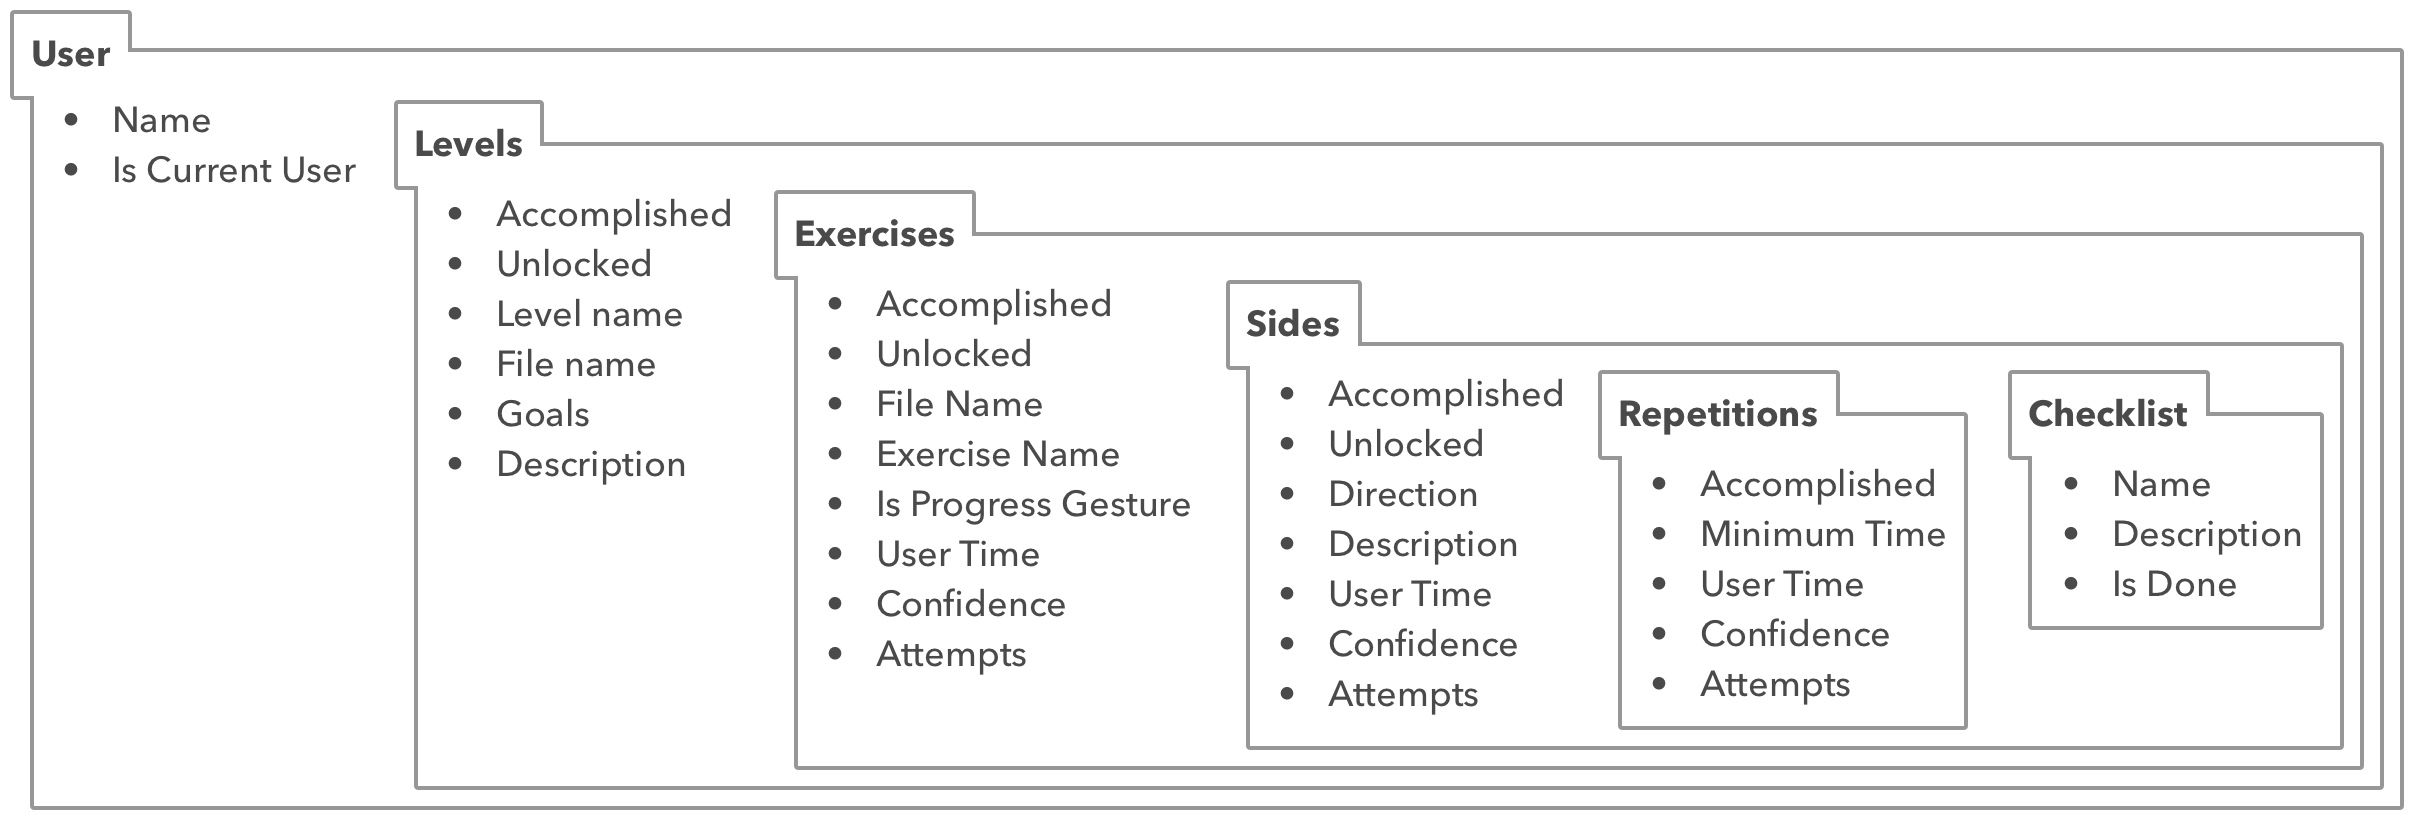
\includegraphics[width=1\linewidth]{Pictures/5_2_dataModel}
		\caption{Data model overview}
		\label{fig:5_2_dataModel}
	\end{minipage}
\end{figure}

%- Name, Side
%-- Side, Description, Min time, Repetitions
%-- Average user time, user attempts, confidence
%-- Checklist
%--- Repetitions
%--- User time, User time, Attempts
%- Average user time, user attempts, confidence
%- Gesture

%This application a 3D project has been generated, since the Kinect uses 3D space to track the user, she should be able to interact within that, and a 3-Dimensional environment design is considered. Further some examples of the interaction implementation is described.

%For each object containing key-value pairs a class is generated, i.e. for Users, Tier, Exercise, Sides, and Repetitions. In listing \todo{ref c\# code example} an example for the \textit{Tier} object can be seen. A class must be marked as serializable to work with the JSON serializer. It contains variables, which match the JSON structure on listing \todo{ref json code}. 
%\todo{c\# code example and json file}

%With this an instance of the class can be created and the value accessed for adjustments (listing \todo{ref img class instance}). This can then be serialized into a JSON object. Line \todo{ln number} shows how existing JSON data can be converted back into an object instance. This is needed to fetch user data that already exists.

%The files are stored within the \textit{StreamingAssets} folder of Unity. Data stored in this folder can easily be accessed via path name of the target machines file system. 
